\documentclass[aspectratio=169]{beamer}

\usetheme{Madrid}
\usecolortheme{default}

\usepackage[russian]{babel}
\usepackage{minted}
\usepackage{hyperref}


\title{Пакеты и библиотеки}
\subtitle{или как правильно использовать чужой код}
\author{Кормышев Егор ИСиП-301}
\date{\today}

\begin{document}

\frame{\titlepage}

% Definition of pocket manager and pocket

\begin{frame}
\frametitle{Термины и определения}

% NPM Package

\textcolor{blue}{\textbf{NPM Пакет}} (или библиотека) -  это набор переиспользуемумого кода опубликованный в \underline{рерозитории}

\bigskip

% Repository

\textcolor{blue}{\textbf{Репозиторий}} - облачное хранилище и система контроля версий для пакетов (сравнимо с github) 
Список пакетов NPM доступен по ссылке \underline{\href{https://www.npmjs.com/}{npmjs.com}}

\bigskip

% NPM

\textcolor{blue}{\textbf{Node Package Manager}} - менеджер пакетов Node.js предоставляющий такие функции для управления пакетами, как \textcolor{blue}{установка}, \textcolor{blue}{удаление}, \textcolor{blue}{редактирование} и другие

\bigskip
\begin{center}
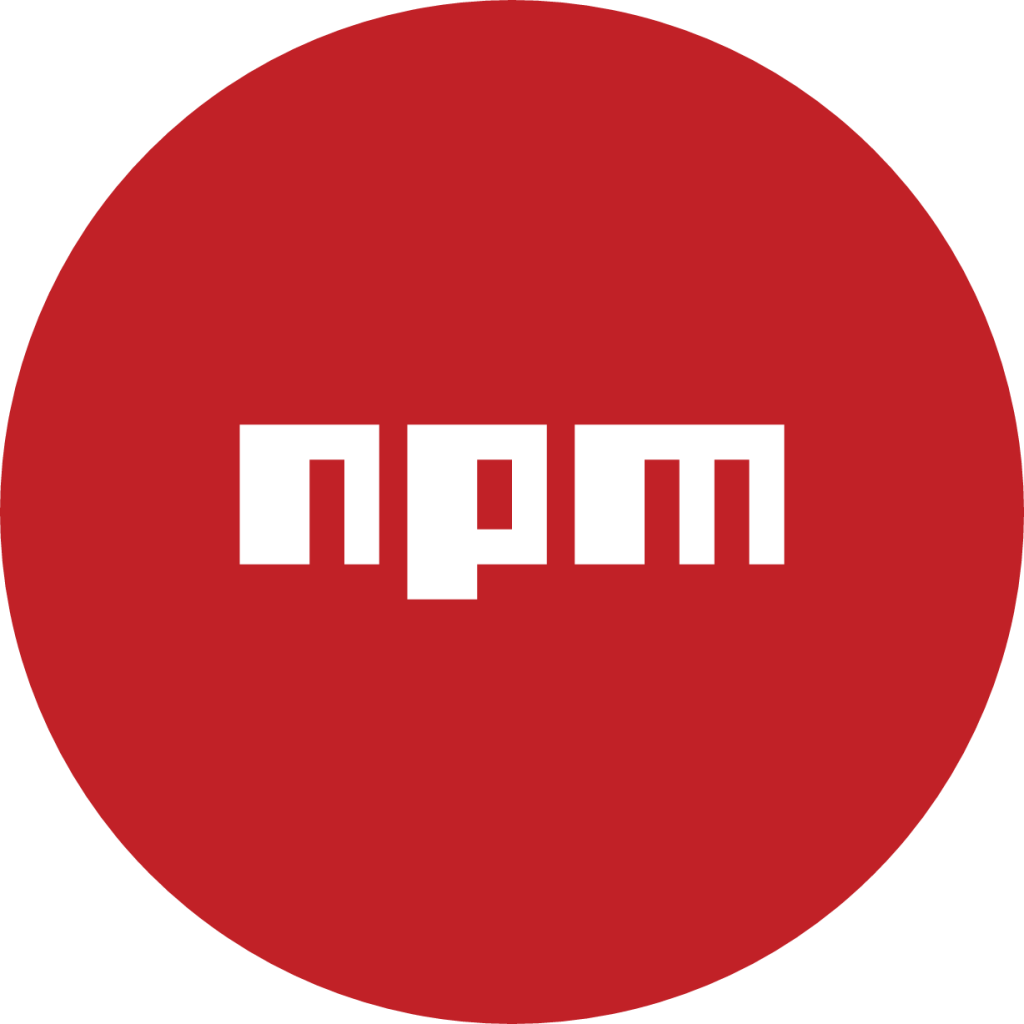
\includegraphics[width=0.2\textwidth]{assets/npmicon.png}
\end{center}

\end{frame}

% Frame 2: Getting started

\begin{frame}
  \frametitle{Начало работы с npm}
  \begin{center}
    \largeДля начала нужно создать новый npm проект 
  \end{center}
  
  \bigskip
  
  Это можно сделать всего в 3 действия:
  \begin{enumerate}
  \item Создать пустую папку
  \item В терминале/консоли перейти в эту папку
  \item Выполнить команду \texttt{npm init}
  \end{enumerate}
\end{frame}

% Frame 3: Interactive project creation

\begin{frame}[fragile,allowframebreaks]
  \frametitle{Создание проекта}
  \begin{center}
    
    \largeС этого момента начинается создание проекта в интерактивном режиме
    NPM поможет вам составить конфигурацию проекта через ответы на вопросы
  \end{center}
  \bigskip
  \begin{center}
    Список вопросов
  \end{center}

  \begin{enumerate}
  \item \texttt{package name} - имя проекта (по умолчанию - имя папки)
  \item \texttt{version} - версия проекта (по умолчанию - 1.0.0)
  \item \texttt{description} - описание - краткое описание назначения и/или функционала проекта
  \item \texttt{entry point} - главный файл проекта (по умолчанию - index.js)
  \item \texttt{test command} - скрипт для тестированя (по умолчанию - просто вывод строки в консоль)
  \item \texttt{git repository} -- ссылка на git репозиторий (при наличии)
  \item \texttt{keywords} - ключевые слова - "теги" по котором будут искать ваш пакет (например: framework, game, preprocessor)
  \item \texttt{author} - автор - ваш ник на npm или github c почтой в особом формате (\texttt{coffeek-codes <kormyshev11@mail.ru>})
  \item \texttt{license} - Лицензия - самая популярная свободная лицензия MIT - подробнее \underline{\href{https://wiki.merionet.ru/articles/sravnenie-open-source-licenzij/}{здесь}}
  \end{enumerate}

  \begin{center}
    Затем вы увидите вашу конфигурацию и последний вопрос с подтверждением.
  \end{center}

  \bigskip
  \bigskip
  \bigskip

  \begin{center}
    \large Поздравляю! Вы создали свой первый npm проект!
  \end{center}
  
\end{frame}

% Frame 4: Exploring created project

\begin{frame}
  \frametitle{Разбираемся с проектом первая зависимость}
\end{frame}

\end{document}
